% !TEX TS-program = pdflatex
% !TEX encoding = UTF-8 Unicode

% This is a simple template for a LaTeX document using the "article" class.
% See "book", "report", "letter" for other types of document.

\documentclass[11pt,twoside]{report} % use larger type; default would be 10pt

\linespread{1}
\renewcommand*\rmdefault{ptm}

\usepackage[utf8]{inputenc} % set input encoding (not needed with XeLaTeX)

%%% Examples of Article customizations
% These packages are optional, depending whether you want the features they provide.
% See the LaTeX Companion or other references for full information.

%%% PAGE DIMENSIONS
\usepackage{geometry} % to change the page dimensions
\geometry{a4paper} % or letterpaper (US) or a5paper or....
\geometry{
	margin=2.5cm,
} % for example, change the margins to 2 inches all round
% \geometry{landscape} % set up the page for landscape
%   read geometry.pdf for detailed page layout information

\usepackage{graphicx} % support the \includegraphics command and options

% \usepackage[parfill]{parskip} % Activate to begin paragraphs with an empty line rather than an indent

%%% PACKAGES
\usepackage{url}
\usepackage{booktabs} % for much better looking tables
\usepackage{array} % for better arrays (eg matrices) in maths
\usepackage{paralist} % very flexible & customisable lists (eg. enumerate/itemize, etc.)
\usepackage{verbatim} % adds environment for commenting out blocks of text & for better verbatim
\usepackage{subfig} % make it possible to include more than one captioned figure/table in a single float
\usepackage[final]{pdfpages}
% These packages are all incorporated in the memoir class to one degree or another...

%%% HEADERS & FOOTERS
\usepackage{fancyhdr} % This should be set AFTER setting up the page geometry
\pagestyle{fancy} % options: empty , plain , fancy
\renewcommand{\headrulewidth}{0pt} % customise the layout...
\lhead{\small Teaching Quantum Mechanics Using qCraft}\chead{}\rhead{\small Micha van den Enk, s1004654}
\lfoot[\small \today]{\small \thepage}
\cfoot{}
\rfoot[\small \thepage]{\small \today}

%%% SECTION TITLE APPEARANCE
\usepackage{sectsty}
\allsectionsfont{\sffamily\mdseries\upshape} % (See the fntguide.pdf for font help)
% (This matches ConTeXt defaults)

%%% RULE

\newcommand{\HRule}{\rule{\linewidth}{0.5mm}}

%%% BIBLIOGRAPHY

\usepackage{apacite}                           %bibliography in apa-style

%%% ToC (table of contents) APPEARANCE
\usepackage[nottoc,notlof,notlot]{tocbibind} % Put the bibliography in the ToC
\usepackage[titles,subfigure]{tocloft} % Alter the style of the Table of Contents
\renewcommand{\cftsecfont}{\rmfamily\mdseries\upshape}
\renewcommand{\cftsecpagefont}{\rmfamily\mdseries\upshape} % No bold!

\setcounter{secnumdepth}{-2}

%%% TABLES

\renewcommand{\arraystretch}{1.2}

\usepackage{afterpage}

\newcommand\blankpage{%
    \null
    \thispagestyle{empty}%
    \newpage}

%%% END Article customizations

%%% The "real" document content comes below...

\begin{document}

\begin{titlepage}

\begin{center}


% Upper part of the page

\includegraphics[width=1\textwidth]{./logo}\\[1cm]    

\textsc{\Large Bachelor Thesis}\\[0.5cm]
\textsc{\Large {[}201000166{]}}\\[0.5cm]


% Title
\HRule \\[0.4cm]
{ \huge \bfseries Literature study}\\[0.4cm]

\HRule \\[1.5cm]

% Author and supervisor
\begin{minipage}{0.4\textwidth}
\begin{flushleft} \large
\emph{Author:}\\
Micha \textsc{van den Enk} \\
{[}s1004654{]} \\
\end{flushleft}
\end{minipage}
\begin{minipage}{0.4\textwidth}
\begin{flushright} \large
\emph{Supervisors:} \\
Dr. H. H. \textsc{Leemkuil} \\
Second \textsc{supervisor} \\
\end{flushright}
\end{minipage}

\vfill

% Bottom of the page
{\large \today}

\end{center}

\end{titlepage}

\afterpage{\blankpage}

\setcounter{tocdepth}{1}
\tableofcontents
\thispagestyle{fancy}
\newpage

\section{Introduction}

The literature study is an important aspect of writing scientific literature, and therefore also relevant for designing educational resources. It contains a description and evaluation of the existing literature relevant to the topic of the study \cite{lerencomm}. For a succesfull literature study, the researcher has to formulate research questions. The answers to these questions can then be used for completing and deepening the analysis.

In the case of designing resources to teach the fundamental principles of quantum mechanics, it is important to look at the different studies which investigate the teaching of quantum mechanics. Hence, the main research question for this literature study is:

\begin{quote} What is known about teaching quantum mechanics from earlier research? \end{quote}
This question leads to several different follow-up questions:

\begin{itemize}
\item What are relevant topics within quantum mechanics education?
\item What are the motivations to teach quantum mechanics?
\item What are the intrinsic difficulties of teaching quantum mechanics?
\item What are the pre-existing conceptions that students have about microscopic phenomena?
\item What are the teaching strategies recommended by the literature?
\item How is quantum mechanics currently taught in secondary education?
\item What are aspects important for implementing quantum mechanics teaching in schools?
\end{itemize}

First, the method will be described which was used to gather the articles, and the method which was used to analyse these articles in a systematic way. This will be followed by a summary of the results from the literature study.

\section{Method}

First, the search terms for the  literature study had to be considered. A quick look on Google Scholar with the terms "quantum mechanics teaching" already yielded many relevant results. Then, the thesaurus from EBSCO Host was consulted to look for relevant similar terms. When looking for "quantum mechanics", the only relevant term which was found was "modern physics", which is the superterm used for both quantum mechanics and relativity theory. Another term similar to quantum mechanics is quantum physics, but because everything quantum related could be relevant, the term used was "quantum*". This resulted in the first search term being "quantum*" OR "modern physics". The term "teaching" could be elaborated by terms like "instruction", "learning" and "education", but this set of terms already became obsolete during the next step, which entails considering the databases.

The first consulted database was ERIC, the database for articles in the field of education. Because the articles within this database are already education related, it was decided to only consider the first set of terms ("quantum*" OR "modern physics"). This results in 1,225 articles. Then, a couple of limiters were applied, which were to search only for articles which were peer reviewed and published in scientific journals and with the full text available. This resulted in 636 articles. After that, a limiter was added to search for articles concerning secondary education only. This yielded 63 articles. Finally, only articles published since 2003 were considered, because quantum mechanics --- especially quantum mechanics teaching --- is a changing field, and articles older then 12 years might not be relevant anymore. With all these limiters --- peer reviewed, published in scientific journals, full text available, secondary education only and published since 2003 --- there were 26 articles left.

Other databases were also consulted, namely Psycinfo, Scopus and Web of Science, with the terms used by ERIC, added by the teaching set and the terms "highschool" OR "secondary education" (("quantum*" OR "modern physics") AND ("teaching" OR "learning" OR "education" OR "instruction) AND ("highschool" OR "secondary education")), but this only yielded a limited amount of results, of which the articles were either irrelevant or already found by using ERIC.

There was one other article found separate from ERIC, written by \citeA{mckagan}. Three articles cited by this article were also added to the collection of consulted articles.

After this, the articles themselves were considered. Four articles were dismissed by title only. These were articles about other topics then quantum mechanics, so they were irrelevant. The rest of the articles were read by abstract, introduction and conclusion. After this, 16 articles contained (partial) answers to the research questions, so the rest of the articles was dismissed as well. After this, a literature matrix was set up with the research questions in one axis and the different articles in the other, and then the cells were filled in by reading the articles thoroughly. The results of this filled in literature matrix will be discussed in the next section.

\section{Results}

\subsection{Topics within quantum mechanics education}

The first logical question which should be asked would be the question which topics exist within the domain of introductory quantum mechanics, because only then we can delve into the question how these topics could or should be thought to novice learners. This exploration would have to start there where the students already familiar with. This is the Rutherford-Bohr Model of the Atom, also known as the Bohr Model, which presents a description of a hydrogen atom (see figure~\ref{fig:bohrmodel}). Students in upper secondary education should at least be familiar with this model, especially those with a technical profile. This gives way to introduce the students to the concept of elementary particles, which are the particles which exhibit quantum behaviour. The Bohr-model is also often referred to in the studied literature \cite{dori, mckagan, muller, papaphotis1, papaphotis2}.

\begin{figure}[h!]
\centering
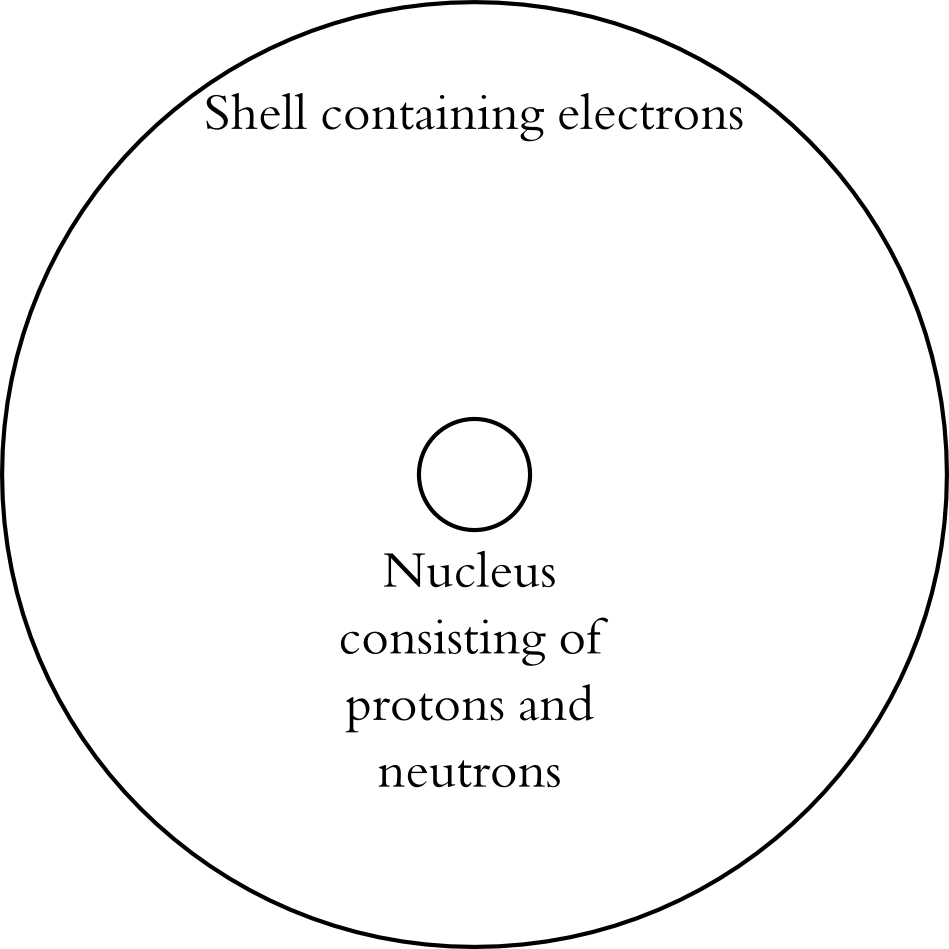
\includegraphics[width=0.5\textwidth]{bohrmodel}
\caption{The Rutherford-Borh Model of the Atom}
\label{fig:bohrmodel}
\end{figure}

Some of the studies \cite{erduran, hubber, muller, thacker} then describe properties of specific elementary particles, mostly of electrons or photons. Often used properties are the photoelectric effect or the polarisation of light \cite{henriksen, mckagan, muller}. These properties could give more meaning to what the elementary particles are and do. Another benefit would be that these properties are used in the various experiments conducted within the field of quantum mechanics.

The double-slit experiment is the most famous of these experiments, and also the most studied tool for educational purposes \cite{asikainen, henriksen, hobson, levrini, mckagan, muller, papaphotis1,singh2, thacker}. A reason why this experiment is famous is because it was the first experiment in history to demonstrate phenomena of quantum mechanics. The experiment entails shooting elementary particles through two narrow slits in a wall, projecting them on a large wall behind these two slits. When the two slits are separated very little, a interference pattern emerges. This is a result expected when the elementary particles would not be particles but waves. However, if the particles are observed and information is available through which slit each particle traversed, a diffraction pattern emerges, which would be the behaviour of particles. The most apparent phenomena demonstrated by this experiment is the wave-particle duality of elementary particles, which then could give way to mathematical descriptions of quantum mechanics like the Schrödinger equation. The Centraal Eindexamen of 2015 also already contained this experiment \cite{eindexamen2015}, so educational resources for teaching this experiment already exist.

For understanding the double-split experiment, the concept of superposition is vital. Superposition means that when a particle is not observed, it is in all possible states at the same time. In the case of the double-slit experiment, superposition means that the particle goes through both slits at the same time. It then interferes with itself because of the probability function of where the particle ends up. However, when the particle is observed through which slit it travels, the information through which slit the particle travels is known and forces the particle to collapse to either the left or the right slit. Because of this, it behaves like a particle and a diffraction pattern emerges. A video which demonstrates the double-slit experiment can be seen on \url{https://upload.wikimedia.org/wikipedia/commons/transcoded/e/e4/Wave-particle_duality.ogv/Wave-particle_duality.ogv.480p.webm}. The double-slit experiment can provide the learner with an explanation of the observer dependency of the elementary particles. However, only \citeA{muller} mentions this concept in his study, and it also does not appear in the Centraal Eindexamen of 2016 \cite{eindexamen2016}.

The concept of superposition also has different cases. There are other properties of elementary particles which can be in superposition, for example the polarity of photons. Upon measurement, the polarisation value of a photon particle collapses to a certain value, but before this collapse it has all the different polarities at the same time. This gives way to the concept of entanglement, mentioned in some researches \cite{henriksen, hobson, kuttner}. Entanglement is a phenomenon which happens between elementary particles, and it has as effect that the collapse of the different particles are interdependent of each other. This entanglement has two forms: boson entanglement and fermion entanglement. When the two particles are bosons, they always collapse to the same state on observation, and when the two particles are fermions, they always collapse to each others opposite state.

Quantum mechanics have led to some fierce debates between scientists \cite{barnes}. Roughly speaking, the scientists could be divided intro two camps: the camp of the realists and the camp of the ontologists. The realists thought that there has to be something underneath quantum mechanics which could explain the strange phenomena of superposition and entanglement, whereas the ontologists thought that the phenomena of quantum mechanics stand on its own. The phenomena of entanglement played a huge role in this debate. The realists first thought that they could use entanglement to prove that there is a reality underneath quantum mechanics, but it eventually led mostly to evidence towards the camp of ontologists. One example of this are Bell's inequalities \cite{kuttner, muller}, which is beyond the scope of this literature study to explain.

\citeA{henriksen} writes that there are three main differences between classical mechanics and quantum mechanics. The first difference is the fact that classical mechanics are deterministic and that quantum mechanics are probabilistic, also brought up by \citeA{levrini} and by \citeA{papaphotis1}. Classical mechanics rely heavily on deterministic causal effects, which can ultimately be explained. This is very apparent in systems of force, where everything moves according to certain laws, the three Newtonian laws for example. Quantum mechanics however relies heavily on probabilistic models, where certain properties of certain elementary particles collapse to certain values in a probabilistic manner.

A second difference between classical mechanics and quantum mechanics mentioned by \citeA{henriksen} is the locality of classical mechanics and the non-locality of quantum mechanics, also mentioned by citeA{hobson}. On the scale of classical mechanic, it is possible to determine the exact position of an object. Well, at least it is possible to do this on a significant scale. Namely, on a very small scale, on the scale of quantum mechanics, the exact position of an object  cannot be determined. There is an inherent uncertainty about the position of an object, which is very small and insignificant on the scale of classical mechanics, but quite significant on the scale of elementary particles. This is also true for the momentum of an elementary particle, which can be translated to the speed of an elementary particle. This uncertainty can be demonstrated by the uncertainty principle of Heisenberg \cite{henriksen, muller, velentzas}, which has as implications that nor the location nor the momentum of an elementary particle can be exactly known and that the more certain the location of an elementary particle is known, the less certain the momentum of an elementary particle can be known and vice versa.

Finally, \citeA{henriksen} mentions that classical mechanics are continuous and that quantum mechanics are discrete. This is because of the Planck length, which is the shortest measurable length. In classical mechanics, this length is very insignificant, and because of that the world looks continuous. A fully continuous world would mean that there is no tiniest unit, but that it is always possible to “go smaller”. For example, if one had a plank of wood, it could be divided in half infinitesimally. However, on a quantum scale, this is not possible, because it is not possible to have something smaller than the Planck length.

Because of the inherent difficulty with quantum mechanics, some scientists have posited thought experiments, which allows the learner to make a mental model about the different concepts of quantum mechanics. The most famous thought experiment is that of Schrödingers cat \cite{muller, velentzas}, where the life of a cat depends on the collapse of an elementary particle. When the cat is then observed, the state of the elementary is observed indirectly, which causes it to collapse and either kill the cat or let the cat live. This teaches the student about observer dependency, the way observations are linked to the random collapse of an elementary particle. Another thought experiment mentioned in the studied literature is the EPR paradox \cite{kuttner, muller, velentzas}, which can be used to teach the student about how entanglement is related to deep questions about the nature of quantum mechanics. This thought experiment however is related to the EPR experiment, which lies beyond the scope of this study to explain.

Finally, there are some studies which recommend certain mathematical approaches to quantum mechanics, namely the Schrödingers equation \cite{muller, singh2}, the Hermitian operator \cite{singh2}, the aforementioned Bell's inequalities \cite{kuttner, muller}, the eigenvalue equation \cite{muller} and the DeBroglie energy levels \cite{dori, gianino, mckagan}. However, these mathematical approaches rely on a thorough conceptual understanding of quantum mechanics and are therefore not relevant to this study.

The topics relevant to teaching quantum mechanics can be summed up as the Rutherford-Bohr model of the Atom and elementary particles, the double-slit experiment, superposition, entanglement, the debate between realists and ontologists, the differences with classical mechanics, thought experiment and the mathematical side of quantum mechanics.

\subsection{Motivations to teach quantum mechanics}

The needs assessment mentions that the need for teaching quantum mechanics exists because of the Centraal Eindexamen. This is an example of extrinsic motivation. However, is there also intrinsic motivation to teach quantum mechanics on high schools? First of all, there is no article which claimed that quantum mechanics should not be taught on high schools. On the other hand there are but a few authors who did have some arguments in favour of teaching. \citeA{muller} and \citeA{henriksen} state that quantum mechanics shapes our world view and that educated citizens should therefore become acquainted with the topic. It is also regarded as fundamental and should therefore be taught \cite{henriksen,hobson}. Finally, \citeA{erduran} states that the teaching of philosophical themes in science education has been advocated for several decades, and quantum mechanics is one of these themes.

\subsection{Intrinsic difficulties of teaching quantum mechanics}

There exists a consensus within the studied articles that quantum mechanics is a difficult topic, and this is also a consensus among educators \cite{gianino,papaphotis1,papaphotis2}. There are a couple of reasons mentioned within the articles to explain this topical difficulty. A couple of sources state that quantum mechanics is a very counter intuitive topic \cite{henriksen, levrini, mckagan, singh2}, because it contradicts a lot of things which are common in daily experience, like locality or determinism. Quantum mechanics is also considered to be a very abstract topic \cite{barnes, gianino, mckagan, papaphotis1, singh1}. Because quantum mechanics differs a lot from our everyday experiences and because of its abstractness, it is difficult for learners to visualise the concepts of quantum mechanics \cite{henriksen, mckagan}. Another factor contributing to the difficulty of quantum mechanics is that it is mathematically challenging \cite{gianino, mckagan}, it involves mathematical skills that most high school students --- even vwo 6 students --- do not possess.

\subsection{Pre-existing conceptions from students about microscopic phenomena}

When developing an instruction, it is important to consider the already available conceptions on the topic. In quantum mechanics, these preconceived models often prove to be incorrect \cite{asikainen, papaphotis2, thacker}. This partly comes from the nature of quantum theory \cite{papaphotis2}, but also partly from textbooks and instruction \cite{hubber, papaphotis2}. The problems often stem from depending on outdated deterministic or realist models \cite{hubber, papaphotis1, papaphotis2}, a often mentioned example of this is that students often mix up the deterministic planetary model with the indeterministic atom model \cite{dori, henriksen, hubber, muller, papaphotis1, papaphotis2}. \citeA{mckagan} also mentions that it is difficult for students to recognise the scale in which quantum mechanics take place.

\citeA{thacker} describes how much knowledge of students consists out of memorised facts, for example that light is a wave and electrons are particles. When the student then is confronted with new or different information from what they know, they develop new memorised facts instead of creating the right model. This then results in models consistent with fragmented models of microscopic processes, which are often incorrect but self-consistent with a certain experiment \cite{hubber, thacker}. When the student cannot model the fragments anymore, this can result in deep skepticism towards quantum mechanics \cite{barnes, henriksen, levrini}. \citeA{muller} has created a long list of exact conceptions students hold about microscopic phenomena, which are too detailed to enlist fully in this article.

\subsection{Teaching strategies}

The literature provides a lot of strategies which can be used to teach quantum mechanics. These can be categorised in four categories. There are recommendations for which content to use. Others describe aspects of the medium used to teach quantum mechanics. Some of the strategies focus on meta-cognitive aspects. Finally, there are a few frameworks which can be used to teach modern physics.

Some of the content-related strategies emphasise the importance of embedding the instruction in real-world contexts, for they help with understanding \cite{mckagan,thacker,dori} and help appreciate the relevance of quantum mechanics \cite{barnes, henriksen, mckagan}. Furthermore, \citeA{thacker} suggests introducing microscopic processes as an integral part of a study of electricity and magnetism. This could help demystify the topic, which also would contribute towards a better understanding \cite{barnes, muller}. An example of how this can be done is by using the e/m experiment, where the electromagnetic effect is demonstrated by the properties of electrons. Furthermore, the language of physics is important \cite{henriksen}, and should be used carefully \cite{mckagan}. The consulted articles all recommend a conceptual approach above a mathematical-oriented approach. Mathematical-oriented approaches might be more common, but most high school students lack proper background in mathematics at the required level \cite{dori}. \citeA{barnes} and \citeA{henriksen} believe teaching through history of science is believed to be constructive.

The recommendations for different aspects of the medium used by the instruction entail interactivity \cite{adegoke, asikainen, dori, mckagan}, visualisation \cite{dori, henriksen, mckagan} (although being done very carefully, because pictures can be misleading \cite{levrini}), the combination of different modes of representation \cite{dori}, and the use of computation \cite{barnes, mckagan, velentzas}. Furthermore, \citeA{mckagan} suggests the use of simulations, as these combine all of the aformentioned aspects.

\citeA{papaphotis1} states that critical thinking skills are crucial for understanding quantum mechanics, because students have to investigate the new material in a critical way to build the correct mental models. Active learning also contributes to investigation of the material. Because the students easily build misconception, right feedback is vital to prevent misconceptions and can stimulate students to build correct mental models. Finally, \citeA{papaphotis1} suggests collaboration, which is also suggested by \citeA{adegoke} and \citeA{barnes}. Collaboration could lead to peers providing each other with critical questions and feedback. Especially in the case of female students this could benefit to learning quantum mechanics \cite{adegoke}. 

The frameworks mentioned by different authors are directly or very similar to thought experiments \cite{asikainen, erduran, levrini, velentzas}. Asikainen describes the most elaborated framework for a well-conducted thought experiment, which includes the steps question and general assumptions, description of the features of the system, performance of the thought experiment itself, extraction of the results and drawing conclusions. \citeA{erduran} and \citeA{levrini} also describe a framework, but the steps they mention already overlap with those of \citeA{asikainen}.

\subsection{Quantum mechanics in current secondary education}

There is a lot of experience with teaching quantum mechanics on high schools. Often, quantum mechanics is introduced with great emphasis on learning and practising algorithmic skills \cite{papaphotis1,papaphotis2}. However, it is also found that students show higher interest in the conceptual aspects than the algorithmic aspects \cite{papaphotis1,papaphotis2,levrini}. When focusing on the conceptual aspects, it engages students \cite{henriksen} and students start asking fundamental questions \cite{mckagan}. Because the usual focus on the algorithmic aspects, students often do not learn what instructors want them to learn \cite{asikainen, mckagan}, and improved student learning is possible by shifting the focus to conceptual understanding \cite{mckagan}.

\subsection{Aspects important for implementing quantum mechanics teaching}

Quantum mechanics teaching is not only difficult for the students learning the topic, but it is also a difficult topic to implement and integrate within high schools. There exists a consensus among the articles that the best way of teaching quantum mechanics is by using new innovations, like computer simulations, as mentioned in the previous section. However, teachers often prefer traditional lectures, because that is easier to implement in their classroom \cite{adegoke}. This difficulty has to be overcome if quantum mechanics is to be taught successfully. Another problem which has to be solved is the fact that teachers themselves also often show to possess a misunderstanding about quantum mechanics \cite{asikainen}. However, experienced teachers who are teaching modern physics are more capable of teaching quantum mechanics \cite{asikainen}.

\section{Conclusion}

There is a wide variety of topics available for quantum mechanics education. Any instruction should start with the Rutherford-Bohr model of the Atom and its relation to elementary particles, for this is the scale on which quantum mechanics take place. A next step could be introducing the different phenomena which happen on a quantum scale, like superposition, observer dependency and entanglement. One way to introduce superposition and observer dependency is by using the double-slit experiment. This also teaches about the wave-particle duality of elementary particles. Furthermore, the students could be taught the differences between classical mechanics and quantum mechanics, which were determinism and probabilism, locality and non-locality, and continuous and discrete distances. One way to highlight the strangeness of quantum mechanics is by using the debate between realism and ontology, this emphasises that quantum mechanics are different than a student might think at first. There are also famous thought experiments like Schrödingers cat, which could be used to create different mental models with the students. Finally, there are some mathematical approaches to quantum mechanics, however there is a consensus within educators that a conceptual approach is more effective.

Not a lot of studies write why quantum mechanics should be taught on secondary education. There is however no study which claimed it should not be taught. Reasons why it should be taught are that educated citizens should be acquainted with quantum mechanics and that it is regarded fundamental.

Quantum mechanics is regarded to be a difficult topic, because it is counter intuitive, it contradicts daily experienced locality and determinism, it is regarded to be abstract, it is difficult to visualise and it is mathematically challenging.

Misconceptions about quantum mechanics can arise out of the nature of quantum theory, but also from textbooks and previous instruction. It is important that the information handed to the students are not simplified, because this can lead to misconceptions. Problems also often originate from outdated deterministic or realist models. The students therefore have to be confronted with the fact that their own models cannot be applied in the context of quantum mechanics. Students also find it difficult to recognise the scale in which quantum mechanics take place. Hence, the students should be informed that quantum mechanics take place on the scale of elementary particles. Knowledge of students often consists out of memorised facts, and when confronted with new or different information, new facts are memorised instead of creating right models. This results in fragmented incorrect but self-consistent models. Because of this, the instruction should provide the student with a coherent description of quantum mechanics.

The literature prescribes different strategies for teaching quantum mechanics, namely recommendations for content, aspects of the medium to use, meta-cognitive aspects and a framework. Content related strategies entail embedding the instruction in real-world contexts, letting the student appreciate the relevance of quantum mechanics, introducing microscopic processes as an integral part of electricity and magnetism, using the language of physics, and using an conceptual approach instead of a mathematical approach. The medium used should be interactive, it should visualise the concepts, it should make use of different modes of representation, and it should make use of computation. It should be noted however that one should be careful with visualisation, for this can easily lead to misconceptions. The use of simulations are suggested. Furthermore, critical thinking skills, active learning, feedback and collaborative learning could contribute to students building the correct mental models of how quantum mechanics work. Finally, thought experiments are regarded to be very effective for learning quantum mechanics, this entails questions and general assumptions, a description of the features of the system, performance of the thought experiment itself, extraction of the results and drawing conclusions.

In secondary education, instructions often emphasise learning and practising algorithmic skills. This however clashes with the recommendations from the literature, which advocates an emphasis on conceptual understanding. It is also found that students show higher interest in conceptual aspects than the algorithmic aspects. Conceptual approaches engage students and probes the student to ask fundamental questions. Because of the focus on algorithmic aspects, student currently often do not learn what is intended by the developer of the instruction, improved student learning might be possible by shifting the focus to conceptual understanding.

Finally, quantum mechanics teaching is a difficult topic to implement and integrate within high schools for two reasons. The literature prescribes the use of new innovations for teaching quantum mechanics, whereas teachers prefer the use of traditional lectures. Because of this, the implementation and use of the software should be made as easy for teachers as possible. Furthermore, a lot of teachers have misconceptions about quantum mechanics themselves. Because of this, it is vital that teachers get instruction about quantum mechanics and its difficulties before they teach it themselves. Experienced teachers who teach modern physics are more capable of teaching quantum mechanics, so they might be used for teaching quantum mechanics to less experienced teachers.

\bibliographystyle{apacite}
\bibliography{references}

\end{document}
